\documentclass[a4paper,12pt]{book}
\usepackage[utf8]{inputenc}
\title{}
\author{Rachel Morris}
\date{\today}

\usepackage{rachwidgets}
\usepackage{fancyhdr}
\usepackage{lastpage}
\usepackage{dirtree}
\usepackage{boxedminipage}

\setcounter{chapter}{7}
\setcounter{section}{1}
\newcommand{\laChapter}{7.2 Proofs about Graphs and Trees\ }

\newcommand{\laClass}{CS 211\ }
\newcommand{\laSemester}{Fall 2017\ }
\newcounter{question}

\pagestyle{fancy}
\fancyhf{}
\lhead{\laClass Exercise, \laSemester}
\chead{}
\rhead{Ch \laChapter}
\rfoot{\thepage\ of \pageref{LastPage}}
\lfoot{\scriptsize Compiled by Rachel Morris, last updated \today}

\renewcommand{\headrulewidth}{2pt}
\renewcommand{\footrulewidth}{1pt}

\begin{document}

    %}\toggletrue{answerkey}
    \togglefalse{answerkey}

    \notonkey{

    %- Team Info ------------------------------------------------------%

    Please write down all people in your team. ~\\

    % table %
    \begin{tabular}{ p{6cm} p{6cm} }
        1. & 2. \\ \\
        3. & 4.
    \end{tabular}
    % table %
    ~\\

    \hrulefill
    }{}

    \section{Proofs about Graphs and Trees}

    Although this section is named ``Proofs", we are actually going to
    focus on Trees for this section.

    \subsection{Introduction to Trees}

% -------------------------------------------------------------%
% - QUESTION --------------------------------------------------%
% -------------------------------------------------------------%
\stepcounter{question}
\begin{question}{\thequestion}{5}
    \footnote{From Jim Van Horn's POGIL Activity 16}
    
    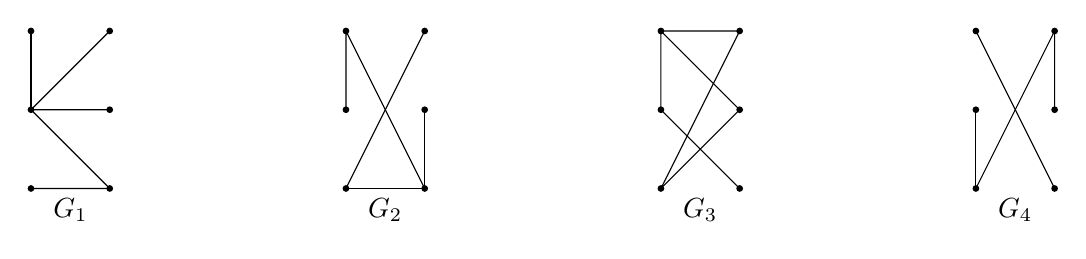
\begin{tikzpicture}
        % Graph 1
        \filldraw (0,0) circle (1pt);
        \filldraw (1,0) circle (1pt);
        \filldraw (0,1) circle (1pt);
        \filldraw (1,1) circle (1pt);
        \filldraw (0,2) circle (1pt);
        \filldraw (1,2) circle (1pt);
        \node[below] at (0.5,0) {$G_{1}$};
        \draw (0,0) -- (1,0) -- (0,1) -- (1,1);
        \draw (0,1) -- (0,2);
        \draw (0,1) -- (1,2);

        % Graph 2
        \filldraw (4,0) circle (1pt);
        \filldraw (5,0) circle (1pt);
        \filldraw (4,1) circle (1pt);
        \filldraw (5,1) circle (1pt);
        \filldraw (4,2) circle (1pt);
        \filldraw (5,2) circle (1pt);
        \node[below] at (4.5,0) {$G_{2}$};
        \draw (4,0) -- (5,0) -- (5,1);
        \draw (4,0) -- (5,2);
        \draw (5,0) -- (4,2) -- (4,1);

        % Graph 3
        \filldraw (8,0) circle (1pt);
        \filldraw (9,0) circle (1pt);
        \filldraw (8,1) circle (1pt);
        \filldraw (9,1) circle (1pt);
        \filldraw (8,2) circle (1pt);
        \filldraw (9,2) circle (1pt);
        \node[below] at (8.5,0) {$G_{3}$};
        \draw (8,0) -- (9,1) -- (8,2) -- (8,1) -- (9,0);
        \draw (8,0) -- (9,2) -- (8,2);

        % Graph 4
        \filldraw (12,0) circle (1pt);
        \filldraw (13,0) circle (1pt);
        \filldraw (12,1) circle (1pt);
        \filldraw (13,1) circle (1pt);
        \filldraw (12,2) circle (1pt);
        \filldraw (13,2) circle (1pt);
        \node[below] at (12.5,0) {$G_{4}$};
        \draw (12,0) -- (12,1);
        \draw (12,0) -- (13,2) -- (13,1);
        \draw (12,2) -- (13,0);
    \end{tikzpicture}

    \begin{itemize}
        \item[a.]   How many vertices does each graph have? ~\\~\\
        \begin{tabular}{p{3cm} p{3cm} p{3cm} p{3cm}}
            $G_{1}$     \solution{ 6 }{ \fitb }
            & $G_{2}$   \solution{ 6 }{ \fitb }
            & $G_{3}$   \solution{ 6 }{ \fitb }
            & $G_{4}$   \solution{ 6 }{ \fitb }
        \end{tabular}

        \item[b.]   How many edges does each graph have? ~\\~\\
        \begin{tabular}{p{3cm} p{3cm} p{3cm} p{3cm}}
            $G_{1}$     \solution{ 5 }{ \fitb }
            & $G_{2}$   \solution{ 5 }{ \fitb }
            & $G_{3}$   \solution{ 6 }{ \fitb }
            & $G_{4}$   \solution{ 4 }{ \fitb }
        \end{tabular} \vspace{0.2cm}
        \item[c.] Which graph is NOT a connected graph?
            \solution{ $G_{4}$ }{}
        \item[d.] Which of the graphs has at least one cycle?
            \solution{ $G_{3}$ }{}
        \item[e.] Which of the graphs is a tree? \solution{ $G_{1}$ and $G_{2}$. }{}
            \begin{hint}{\ }
                A simple connected graph with no cycles is a \textbf{tree}.
            \end{hint}
    \end{itemize}

\end{question}

\notonkey{ \newpage }{ \hrulefill }

% -------------------------------------------------------------%
% - QUESTION --------------------------------------------------%
% -------------------------------------------------------------%
\stepcounter{question}
\begin{question}{\thequestion}{2}
    \footnote{From Jim Van Horn's POGIL Activity 16}
    
    \begin{center}
        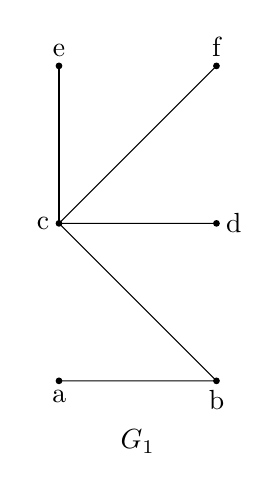
\begin{tikzpicture}
        % Graph 1
        \filldraw (0,0) circle (1pt) node[below] {a};
        \filldraw (2,0) circle (1pt) node[below] {b};
        \filldraw (0,2) circle (1pt) node[left] {c};
        \filldraw (2,2) circle (1pt) node[right] {d};
        \filldraw (0,4) circle (1pt) node[above] {e};
        \filldraw (2,4) circle (1pt) node[above] {f};
        \node[below] at (1,-0.5) {$G_{1}$};
        \draw (0,0) -- (2,0) -- (0,2) -- (2,2);
        \draw (0,2) -- (0,4);
        \draw (0,2) -- (2,4);
    \end{tikzpicture}
    \end{center}

    \begin{itemize}
        \item[a.]   What is the degree of each of the vertices in $G_{1}$?
        ~\\~\\~\\
        \begin{tabular}{p{4cm} p{4cm} p{4cm}}
            $deg(a)$    \solution{ 1 }{ \fitb }
            & $deg(b)$  \solution{ 2 }{ \fitb }
            & $deg(c)$  \solution{ 4 }{ \fitb }
            \\ \\ \\
            $deg(d)$    \solution{ 1 }{ \fitb }
            & $deg(e)$  \solution{ 1 }{ \fitb }
            & $deg(f)$  \solution{ 1 }{ \fitb }
        \end{tabular} \notonkey{ \vspace{1cm} }{}

        \item[b.]   List the leaves for $G_{1}$. \solution{ a, d, e, f }{}
            \begin{hint}{\ }
                Vertices of degree 1 in a tree are called \textbf{leaves} of the tree.
            \end{hint}
            
    \end{itemize}
    
\end{question}

\notonkey{ \newpage }{ \hrulefill }

\notonkey{
\begin{intro}{\ }
    A \textbf{Tree} is a connected simple graph that has no cycles.
    Vertices of degree 1 in a tree are called \textbf{Leaves} of the tree.
    \footnote{Discrete Mathematics, Ensley and Crawley}
\end{intro}
}{}

% -------------------------------------------------------------%
% - QUESTION --------------------------------------------------%
% -------------------------------------------------------------%
\stepcounter{question}
\begin{question}{\thequestion}{4}
    \footnote{From Jim Van Horn's POGIL Activity 16}

    Given these 6 vertices, draw a tree other than $G_{1}$ or $G_{2}$.
    
    \begin{center}
        \begin{tikzpicture}
        % Graph 1
        \filldraw (0,0) circle (1pt) node[below] {a};
        \filldraw (2,0) circle (1pt) node[below] {b};
        \filldraw (0,2) circle (1pt) node[left] {c};
        \filldraw (2,2) circle (1pt) node[right] {d};
        \filldraw (0,4) circle (1pt) node[above] {e};
        \filldraw (2,4) circle (1pt) node[above] {f};
    \end{tikzpicture}
    \end{center}

    \solution{Multiple solutions}{}

    \begin{itemize}
        \item[a.]   How many edges are in your new tree?
            \solution{ 5 }{ \vspace{1cm} }
            
        \item[b.]   How many leaves on your new tree?
            \solution{ 3 }{ \vspace{1cm} }
            
        \item[c.]   If you removed one edge, would the graph still be connected?
            \solution{ no }{ \vspace{1cm} }
    \end{itemize}
    
\end{question}

\notonkey{
\begin{intro}{\ }
    A tree with $n$ vertices will have $n-1$ edges. In other words,
    it is a connected graph and if you remove an edge then it will
    become a disconnected graph.
\end{intro}
}{}

\notonkey{ \newpage }{ \hrulefill }

\subsection{Subgraphs and Trees}

\notonkey{
\begin{intro}{\ }
    A graph $H$ is a \textbf{subgraph} of a graph $G$ if all nodes
    and edges in $H$ are also nodes and edges in $G$.
    \footnote{Discrete Mathematics, Ensley and Crawley}
\end{intro}
}{}

% -------------------------------------------------------------%
% - QUESTION --------------------------------------------------%
% -------------------------------------------------------------%
\stepcounter{question}
\begin{question}{\thequestion}{4}
    \footnote{From Jim Van Horn's POGIL Activity 16}
    
        \begin{tikzpicture}
        \filldraw (1,0) circle (1pt) node[below]    {9};
        \filldraw (2,0) circle (1pt) node[below]    {10};
        \filldraw (1,2) circle (1pt) node[left]     {5};
        \filldraw (2,2) circle (1pt) node[right]    {6};
        \filldraw (1,4) circle (1pt) node[above]    {1};
        \filldraw (2,4) circle (1pt) node[above]    {2};
        \filldraw (0,1) circle (1pt) node[left]     {7};
        \filldraw (3,1) circle (1pt) node[right]    {8};
        \filldraw (0,3) circle (1pt) node[left]     {3};
        \filldraw (3,3) circle (1pt) node[right]    {4};
        \draw (1,0) -- (2,0) -- (3,1) -- (2,2) -- (3,3) -- (2,4) -- (1,4) -- (0,3) -- (1,2) -- (0,1) -- (1,0);
        \draw (1,0) -- (2,2) -- (1,4);
        \draw (2,0) -- (1,2) -- (2,4);
        \node[below] at (1.5,-0.5) {$G$};
        \node[below] at (6,-0.5) {$G_{1}$};
        \node[below] at (10,-0.5) {$G_{2}$};
    \end{tikzpicture}

    \begin{itemize}
        \item[a.]   Draw a graph $G_{1}$ above using vertices and edges from $G$...\\
            Vertices: 1, 2, 5, \tab
            Edges: \{1, 2\} and \{2, 5\}.  \\ \\
            Is this a \textbf{subgraph}?                        \solution{ Yes }{ \vspace{0.5cm} } \\
            Are all the vertices of $G_{1}$ also nodes of $G$?  \solution{ Yes }{ \vspace{0.5cm} }  \\
            Are all the edges of $G_{1}$ also edges of $G$?     \solution{ Yes }{ \vspace{0.5cm} }
            
            
        \item[b.]   Draw a graph $G_{2}$ above using vertices and edges from $G$...\\
            Vertices: 1, 3, 4, \tab
            Edges: \{1, 3\} and \{3, 4\} \\ \\
            Is this a \textbf{subgraph}?                        \solution{ No }{ \vspace{0.5cm} } \\
            Are all the vertices of $G_{2}$ also nodes of $G$?  \solution{ Yes }{ \vspace{0.5cm} }  \\
            Are all the edges of $G_{2}$ also edges of $G$?     \solution{ No }{ \vspace{0.5cm} }
            
    \end{itemize}
    
\end{question}

\notonkey{ \newpage }{ \hrulefill }

\subsection{Spanning Trees}

\notonkey{
\begin{intro}{\ }
    Let $G$ be a simple connected graph. The subgraph $T$ is a
    \textbf{spanning tree} of $G$ if $T$ is a tree and every node
    in $G$ is a node in $T$.
    \footnote{Discrete Mathematics, Ensley and Crawley}

\paragraph{Example:}
    \footnote{From Jim Van Horn's POGIL Activity 16}

    \begin{center}
        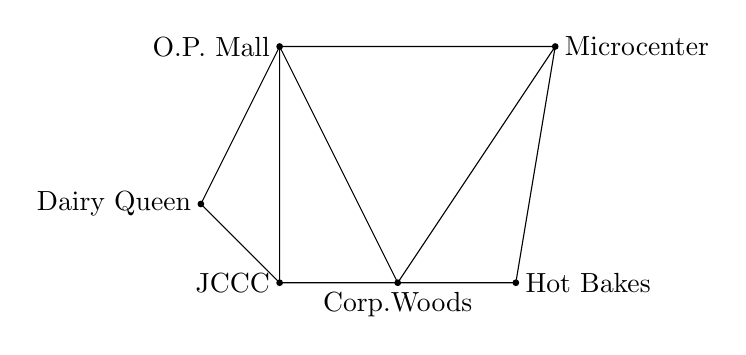
\begin{tikzpicture}
            \filldraw (0,0) circle (1pt) node[left]     {JCCC};
            \filldraw (-1,1) circle (1pt) node[left]    {Dairy Queen};
            \filldraw (1.5,0) circle (1pt) node[below]  {Corp.Woods};
            \filldraw (3,0) circle (1pt) node[right]    {Hot Bakes};
            \filldraw (0,3) circle (1pt) node[left]     {O.P. Mall};
            \filldraw (3.5,3) circle (1pt) node[right]    {Microcenter};
            \draw (0,0) -- (-1,1) -- (0,3) -- (3.5,3) -- (3,0) -- (1.5,0) -- (0,0) -- (0,3) -- (1.5,0) -- (3.5,3);
        \end{tikzpicture}
    \end{center}

    To get from Corporate Woods to JCCC, there are three paths leading into JCCC:
    
    (1) Directly from CW $\to$ JCCC,

    (2) CW $\to$ OP Mall $\to$ JCCC, and
    
    (3) CW $\to$ OP Mall $\to$ Dairy Queen $\to$ JCCC

    ~\\
    We want to make a graph that connects all locations with the fewest paths.
    One way to do this is to remove edges of a cycle until no additional edges
    can be removed without getting a disconnected graph.

    One example result is this:
    
    \begin{center}
        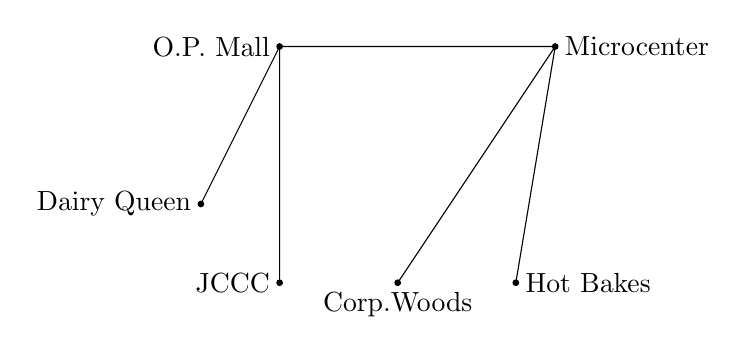
\begin{tikzpicture}
            \filldraw (0,0) circle (1pt) node[left]     {JCCC};
            \filldraw (-1,1) circle (1pt) node[left]    {Dairy Queen};
            \filldraw (1.5,0) circle (1pt) node[below]  {Corp.Woods};
            \filldraw (3,0) circle (1pt) node[right]    {Hot Bakes};
            \filldraw (0,3) circle (1pt) node[left]     {O.P. Mall};
            \filldraw (3.5,3) circle (1pt) node[right]    {Microcenter};
            \draw (-1,1) -- (0,3) -- (0,0);
            \draw (0,3) -- (3.5,3) -- (1.5, 0);
            \draw (3.5, 3) -- (3,0);
        \end{tikzpicture}
    \end{center}

\end{intro}
}{}

\notonkey{ \newpage }{ \hrulefill }

\notonkey{
\begin{intro}{\ }
    \textbf{Spanning Tree algorithm}
    \footnote{Discrete Mathematics, Ensley and Crawley}
    \begin{enumerate}
        \item   Begin with a simple connected graph $G_{0}$.
        \item   For each $i \geq 1$, as long as there is a cycle in $G_{i-1}$...
        \begin{enumerate}
            \item   Choose an edge $e$ in any cycle of $G_{i-1}$, and form the subgraph $G_{i}$
            of $G_{i-1}$ by deleting $e$ from $G_{i-1}$
        \end{enumerate}
        \item   The final result $G_{k}$ will be a spanning tree of $G_{0}$. This is a spanning tree.
    \end{enumerate}
\end{intro}
}{}


% -------------------------------------------------------------%
% - QUESTION --------------------------------------------------%
% -------------------------------------------------------------%
\stepcounter{question}
\begin{question}{\thequestion}{2}

    Follow the algorithm to create a Spanning Tree from this map.
    ``x" out edges that you choose to delete as you go. Draw your
    spanning tree below.
    
    \begin{center}
        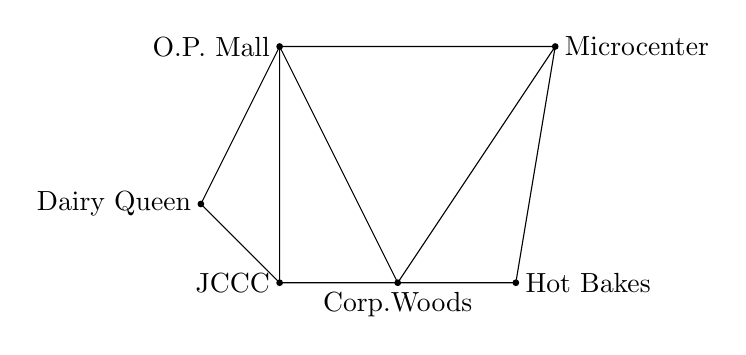
\begin{tikzpicture}
            \filldraw (0,0) circle (1pt) node[left]     {JCCC};
            \filldraw (-1,1) circle (1pt) node[left]    {Dairy Queen};
            \filldraw (1.5,0) circle (1pt) node[below]  {Corp.Woods};
            \filldraw (3,0) circle (1pt) node[right]    {Hot Bakes};
            \filldraw (0,3) circle (1pt) node[left]     {O.P. Mall};
            \filldraw (3.5,3) circle (1pt) node[right]    {Microcenter};
            \draw (0,0) -- (-1,1) -- (0,3) -- (3.5,3) -- (3,0) -- (1.5,0) -- (0,0) -- (0,3) -- (1.5,0) -- (3.5,3);
        \end{tikzpicture}
    \end{center}

    \solution{Multiple solutions}{}
    
\end{question}

\notonkey{ \newpage }{ \hrulefill }

\subsection{Minimal Spanning Trees}

\notonkey{
\begin{intro}{\ }
    \textbf{Prim's Minimal Spanning Tree algorithm}
    \footnote{Discrete Mathematics, Ensley and Crawley}
    \begin{enumerate}
        \item   Given a connected simple graph $G$ with $n+1$ nodes.
        \item   Let $v_{0}$ be any node in $G$, and let $T_{0} = \{v_{0}\}$
                be a tree with one node and no edges.
        \item   For each $k$ from $\{1, 2, ..., n\}$...
        \begin{enumerate}
            \item   Let $E_{k} = \{e$ an edge in $G$ : $e$ has one endpoint in $T_{k-1}$ and
                    the other endpoint not in $T_{k-1}\}$.
            \item   Let $e_{k}$ be the edge in $E_{k}$ with the smallest weight.
                    (In case of a tie, choose any edge of the smallest weight.)
            \item   Let $T_{k}$ be the tree obtained by adding edge $e_{k}$
                    (along with its node not already in $T_{k-1}$ to $T_{k-1}$.
        \end{enumerate}
        \item   $T_{n}$ is the tree returned by the algorithm.
    \end{enumerate}
\end{intro}
}{}

% -------------------------------------------------------------%
% - QUESTION --------------------------------------------------%
% -------------------------------------------------------------%
\stepcounter{question}
\begin{question}{\thequestion}{2}

    % 7.2 Example 6

    \begin{center}
        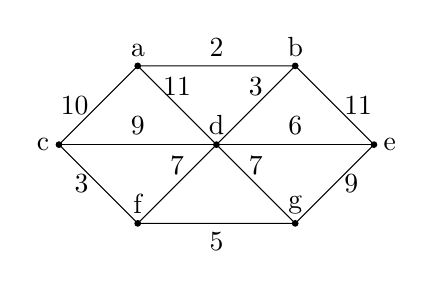
\begin{tikzpicture}
            \filldraw (-1,  1)  circle (1pt)    node[above]     {a};
            \filldraw (1,   1)  circle (1pt)    node[above]     {b};
            \filldraw (-2,  0)  circle (1pt)    node[left]      {c};
            \filldraw (0,   0)  circle (1pt)    node[above]     {d};
            \filldraw (2,   0)  circle (1pt)    node[right]     {e};
            \filldraw (-1,  -1) circle (1pt)    node[above]     {f};
            \filldraw (1,   -1) circle (1pt)    node[above]     {g};
            \draw (-1,1)
                -- node[pos=0.5,above]  {2} (1,1)
                -- node[pos=0.5,right]  {11} (2,0)
                -- node[pos=0.5,right]  {9} (1,-1)
                -- node[pos=0.5,below]  {5} (-1,-1)
                -- node[pos=0.5,left]   {3} (-2,0)
                -- node[pos=0.5,left]   {10} (-1,1);
            \draw (-1,1)
                -- node[pos=0.5,above] {11} (0, 0)
                -- node[pos=0.5,above] {7} (1, -1);
            \draw (-1,-1)
                -- node[pos=0.5,above] {7} (0, 0)
                -- node[pos=0.5,above] {3} (1, 1);
            \draw (-2, 0)
                -- node[pos=0.5,above] {9} (0, 0)
                -- node[pos=0.5,above] {6} (2, 0);
        \end{tikzpicture}
    \end{center}
    
    Use Prim's algorithm to find a minimal spanning tree for the graph.

    \solution{
        Multiple solutions depending on which node you start at, but for example...

        \begin{tabular}{p{3cm} p{3cm} p{3cm} p{3cm} }
            1. & 2. & 3. & 4.
            \\
            \begin{tikzpicture}
                \filldraw(-1,1) circle (1pt) node [above] {a};
            \end{tikzpicture}
            &
            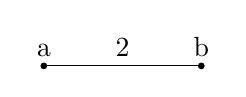
\begin{tikzpicture}
                \filldraw(-1,1) circle (1pt) node [above] {a};
                \filldraw(1,1) circle (1pt) node [above] {b};
                \draw (-1,1) -- node[pos=0.5,above] {2} (1,1);
            \end{tikzpicture}
            &
            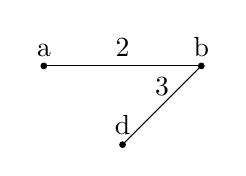
\begin{tikzpicture}
                \filldraw(-1,1) circle (1pt) node [above] {a};
                \filldraw(1,1) circle (1pt) node [above] {b};
                \filldraw (0,   0)  circle (1pt)    node[above]     {d};
                \draw (-1,1) -- node[pos=0.5,above] {2} (1,1);
                \draw (1,1) -- node[pos=0.5,above] {3} (0,0);
            \end{tikzpicture}
            &
            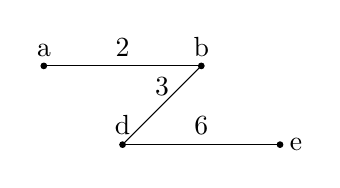
\begin{tikzpicture}
                \filldraw(-1,1) circle (1pt) node [above] {a};
                \filldraw(1,1) circle (1pt) node [above] {b};
                \filldraw (0,   0)  circle (1pt)    node[above]     {d};
                \filldraw (2,   0)  circle (1pt)    node[right]     {e};
                \draw (-1,1) -- node[pos=0.5,above] {2} (1,1);
                \draw (1,1) -- node[pos=0.5,above] {3} (0,0);
                \draw (0,0) -- node[pos=0.5,above] {6} (2,0);
            \end{tikzpicture}
        \end{tabular}
        
        \begin{tabular}{p{6cm}  p{6cm} }
            5. & 6.
            \\
            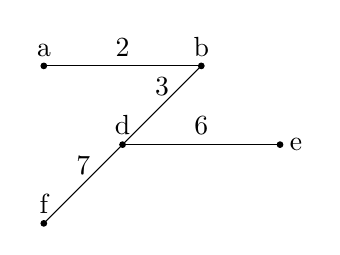
\begin{tikzpicture}
                \filldraw(-1,1) circle (1pt) node [above] {a};
                \filldraw(1,1) circle (1pt) node [above] {b};
                \filldraw (0,   0)  circle (1pt)    node[above]     {d};
                \filldraw (-1,  -1) circle (1pt)    node[above]     {f};
                \filldraw (2,   0)  circle (1pt)    node[right]     {e};
                \draw (-1,1) -- node[pos=0.5,above] {2} (1,1);
                \draw (1,1) -- node[pos=0.5,above] {3} (0,0);
                \draw (0,0) -- node[pos=0.5,above] {7} (-1,-1);
                \draw (0,0) -- node[pos=0.5,above] {6} (2,0);
            \end{tikzpicture}
            &
            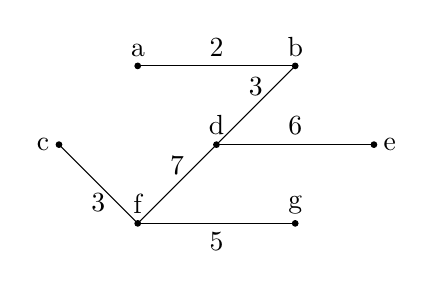
\begin{tikzpicture}
                \filldraw(-1,1) circle (1pt) node [above] {a};
                \filldraw(1,1) circle (1pt) node [above] {b};
                \filldraw (0,   0)  circle (1pt)    node[above]     {d};
                \filldraw (-1,  -1) circle (1pt)    node[above]     {f};
                \filldraw (-2,  0)  circle (1pt)    node[left]      {c};
                \filldraw (2,   0)  circle (1pt)    node[right]     {e};
                \filldraw (1,   -1) circle (1pt)    node[above]     {g};
                \draw (-1,1) -- node[pos=0.5,above] {2} (1,1);
                \draw (1,1) -- node[pos=0.5,above] {3} (0,0);
                \draw (0,0) -- node[pos=0.5,above] {7} (-1,-1);
                \draw (0,0) -- node[pos=0.5,above] {6} (2,0);
                \draw (-1,-1) -- node[pos=0.5,below] {3} (-2,0);
                \draw (-1,-1) -- node[pos=0.5,below] {5} (1,-1);
            \end{tikzpicture}
            \\ \\ 7. \\
            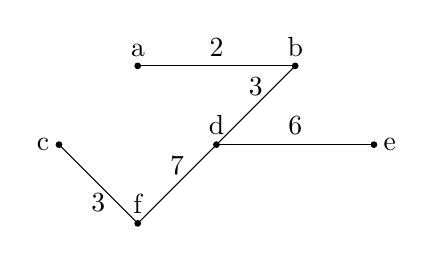
\begin{tikzpicture}
                \filldraw(-1,1) circle (1pt) node [above] {a};
                \filldraw(1,1) circle (1pt) node [above] {b};
                \filldraw (0,   0)  circle (1pt)    node[above]     {d};
                \filldraw (-1,  -1) circle (1pt)    node[above]     {f};
                \filldraw (-2,  0)  circle (1pt)    node[left]      {c};
                \filldraw (2,   0)  circle (1pt)    node[right]     {e};
                \draw (-1,1) -- node[pos=0.5,above] {2} (1,1);
                \draw (1,1) -- node[pos=0.5,above] {3} (0,0);
                \draw (0,0) -- node[pos=0.5,above] {7} (-1,-1);
                \draw (0,0) -- node[pos=0.5,above] {6} (2,0);
                \draw (-1,-1) -- node[pos=0.5,below] {3} (-2,0);
            \end{tikzpicture}
        \end{tabular}
    }{}
    
\end{question}



\end{document}
